\chapter{Experiments and results}

\label{sec:experiments}

This chapter describes the experiments which have been conducted in order to measure the performance of the obstacle detection algorithm. These experiments include tests in a computer-generated environment as well as real-world tests on the robot platform. For the computer-generated environment quantitative measures describing the performance of the algorithm have been developed.

\section{Environments}

In this section the environments used for testing the algorithm are described. Those environments cover two computer-generated scenes and a real-world test in a living room inspired test room.

\subsection{Computer-generated environments}

\begin{figure}[p]
 \begin{center}
  \subbottom[Apartment scene ($7 \times 5 \; \mathrm{m}$)]{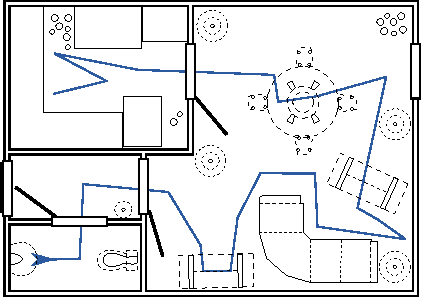
\includegraphics[width=0.6\textwidth]{media/flat_outlines.pdf}}
  \subbottom[Laboratory scene ($10 \times 10 \; \mathrm{m}$)]{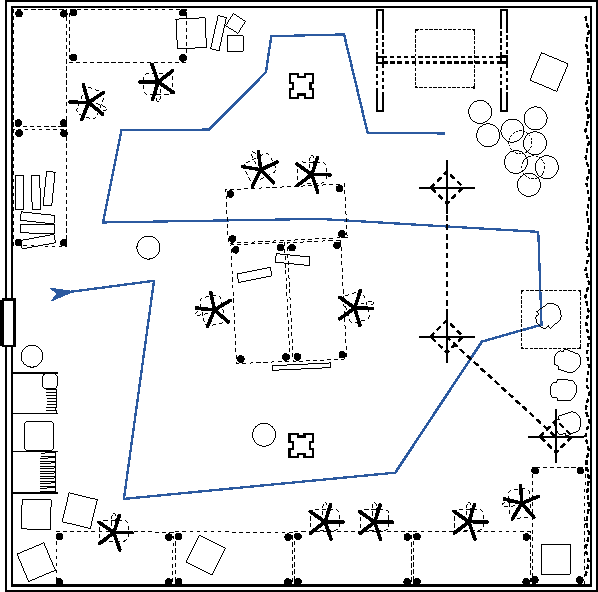
\includegraphics[width=0.85\textwidth]{media/laboratory_outlines.pdf}}
 \end{center}
 \caption{Overview of the computer-generated scenes. Solid lines indicate obstacles relevant to the robot (as they are placed directly on the floor), dashed lines are only for orientation and indicate objects which are too high to be detected as obstacles. The blue line depicts the robot trajectory.}
 \label{fig:floorplan}
\end{figure}

\begin{figure}[t]
 \begin{center}
  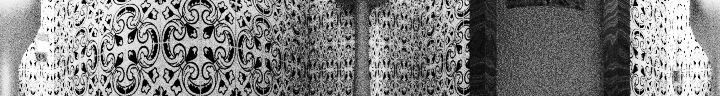
\includegraphics[width=0.49\textwidth]{media/sample_snapshots/flat4.png}
  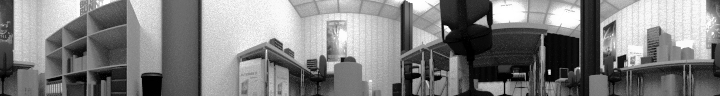
\includegraphics[width=0.49\textwidth]{media/sample_snapshots/lab1.png}
  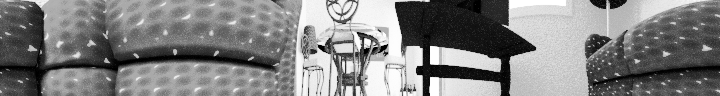
\includegraphics[width=0.49\textwidth]{media/sample_snapshots/flat1.png}
  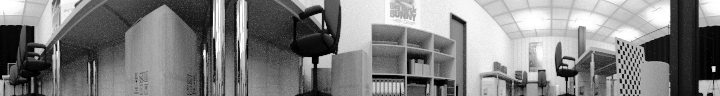
\includegraphics[width=0.49\textwidth]{media/sample_snapshots/lab2.png}
  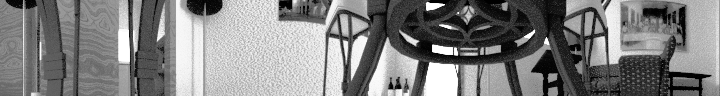
\includegraphics[width=0.49\textwidth]{media/sample_snapshots/flat2.png}
  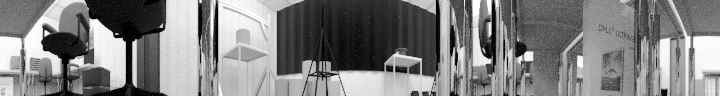
\includegraphics[width=0.49\textwidth]{media/sample_snapshots/lab3.png}
  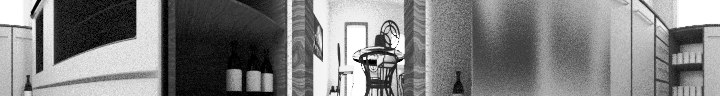
\includegraphics[width=0.49\textwidth]{media/sample_snapshots/flat3.png}
  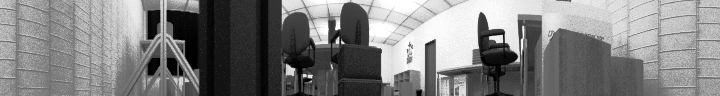
\includegraphics[width=0.49\textwidth]{media/sample_snapshots/lab4.png}
 \end{center}
 \caption{Some exemplary snapshots from the apartment scene (left) and the laboratory scene (right) with applied histogram equalization. The pictures are used as input for the test runs exactly as shown here.}
 \label{fig:sample_snapshots}
\end{figure}

Measuring a perfect ground truth for the depth reconstruction stage of the algorithm in the real-world would be a very tedious task. In computer-generated environments, the ground truth can be simply extracted by storing the so-called $z$-buffer, which contains the distance of each pixel in the scene and is created during the rendering process. Moreover, the computer-generated scenes allow to test the algorithm under a perfect path integration assumption (section \ref{sec:assumptions}) as the position and orientation of the robot are known at all times.

The algorithm is given a sequence of prerendered panoramic snapshot images. These snapshots are generated from the perspective of a virtual robot which moves with constant velocity along a predefined trajectory. The trajectories were laid out by hand, no navigation or obstacle evasion was simulated.

The scenes were modeled and rendered using the open-source software \textit{Blender} and its path-tracing renderer \textit{Cycles}\footnote{See \url{http://www.blender.org/} for more information.}, which was slightly modified in order to produce the required spherical panoramic images. The scenes were rendered under full global illumination. The snapshot resolution is set to $720 \times 96$ pixels and the depression and elevation angles are set to $\check \gamma = 0^\circ$ and $\hat \gamma = 30^\circ$, respectively. The robot travels along the trajectory at $0.2 \, \frac{\mathrm{m}}{\mathrm{s}}$. A new frame is created every $200 \, \mathrm{ms}$. The virtual camera moves at an elevation of $0.1 \; \mathrm{m}$ above the floor. Note that the images contain sampling noise produced by the path-tracer.

Two environments (see figure \ref{fig:sample_snapshots} for example images) were created: A large-scale single-room laboratory scene and a relatively small apartment scene, consisting of bathroom, hallway, living room and a kitchen. See figure \ref{fig:floorplan} for the scene layouts. 

The laboratory scene primarily features two types of table legs (cylindrical brushed metal legs and rectangular dull-white powder-coated legs), chairs, printed cardboard boxes, tripod legs and featureless cylinders as obstacles. Two of the walls (left and right) feature a very fine wallpaper-like structure, the other two walls feature a brick texture. The scene is lit by a total of nine ceiling lights. In order to simulate a realistic computer scientist working environment, the window openings are barred with a light-tight black curtain. The average distance between the robot and the obstacles is relatively high (typically around $\approx 0.5 - 1 \, \mathrm{m}$). The prerecorded trajectory consists of $873$ snapshot images.

The apartment scene features floor lamps, a couch, tables, chairs, bathroom and kitchen interior as well as empty glass bottles in the corners of the room\footnote{The author likes to stress that the apartment scene in no way reflects his own living environment.}. The bathroom is tiled with patterned tiles, while the other walls in the apartment are covered with relatively rough interior wall plaster. The scene is lit through various window openings. The average distance between the camera and the obstacles is relatively small (typically around $\approx 0.2-0.6\,\mathrm{m}$). The prerecorded trajectory consists of $624$ snapshot images.

While the resulting snapshots are not completely photo-realistic, they are believed to be a reasonable approximation.

\subsection{Real-world tests}

Real-world tests are performed on the actual mobile robot platform which runs the fully optimized version of the obstacle detection algorithm. The robot performs a cleaning run in which it seeks to drive parallel lanes in order to cover the complete room. The detected obstacle points are directly fed into the navigation algorithm and influence the robot trajectory. The robot captures a snapshot image approximately every $200 \, \mathrm{ms}$ and moves at a translatory velocity of about $0.2 \, \frac{\mathrm{m}}{\mathrm{s}}$.

The obstacle detection is activated whenever the robot drives straight lanes. It fully relies on odometry data as input for the local motion parameters. In the current implementation, the motion parameters are not integrated between the snapshots. The wheel encoder values are read after an image has been captured and are assumed to be piecewise linear. The odometry data and the snapshot images are recorded for later analysis.

The test room features a living room suite (four chairs, one table, carpet on the floor), a couch, floor lamp, curtain and a sideboard. The room is lit by a single fluorescent ceiling lamp. The floor of the room is covered with wooden planks leading to a slightly uneven floor.

\section{Quality measures}

The simulated test runs are analyzed using quantitative quality measures. These include the count of \textit{true} and \textit{false positive} obstacle points as well as the average obstacle point detection error and the average depth reconstruction error.

\subsection{True and false positive obstacle points}
Let $\img{M_R}$ denote the local environment map as generated by the algorithm containing the reconstructed obstacle points and let $\img{M_T}$ be a reference local environment map, which --- instead of using the reconstructed depth map --- is generated from the ground truth depth map. Note that the depth variance $\sigma_r$ used in the generation of $\img{M_T}$ has to be chosen as a constant value describing the quantization error of the reference depth map (the depth is sampled at 8 bit with a resolution of $0.078 \, \nicefrac{\mathrm{m}}{\mathrm{dig}}$). Additionally, the following sets need to be defined:
\begin{align*}
  P_R &:= \{ \vec p = (x, y)^T \mid \vec p \text{ is reconstructed obstacle point in } \img{M_R}\} \\
  P_T &:=  \{ \vec q = (x, y)^T \mid \vec q \text{ is true obstacle point in } \img{M_T}\}
\end{align*}
where $\vec p$ and $\vec q$ denote the obstacle points in Cartesian world coordinates. Furthermore the function
\begin{equation}
  \mathcal{D}(\vec p; A) := \min \left\{\| \vec p - \vec q \| \mid \vec q \in A \right\}
\end{equation}
denotes the distance between $\vec p$ and the point $\vec q \in A$ closest to $\vec p$.

Given a threshold value $\chi$, define the following sets, which describe \textit{true positive} obstacle points (reconstructed obstacle points near a true obstacle point) and \textit{false positive} obstacle points (reconstructed obstacle points having no near true obstacle point).
\begin{align}
\begin{aligned}
  T_{\mathrm{POS}} &:= \{\vec p \in P_R \mid \mathcal{D}(\vec p; P_T) < \chi\} \; ,\\
  F_{\mathrm{POS}} &:= \{\vec p \in P_R \mid \mathcal{D}(\vec p; P_T) \geq \chi\} \; .
\end{aligned}
\end{align}
For the experiments $\chi$ is arbitrarily chosen as the radius of the robot platform ($\chi = 0.15\,\mathrm{m}$). Note that smaller values (for example $\chi = 0.05\,\mathrm{m}$) might allow for a better evaluation of the algorithm's performance, yet due to limited time, the evaluation of the experiments presented here was not repeated. However, the expressiveness of the results suffices for qualitative statements regarding false and true positive obstacle count.

The two measures describing the obstacle detection performance are given as
\begin{align}
\begin{aligned}
  \nu_F &= \frac{|F_{\mathrm{POS}}|}{|P_R|} \; ,&
  \nu_T &= \frac{|T_{\mathrm{POS}}|}{|P_T|} \; ,
\end{aligned}
\end{align}
where $\nu_F$ corresponds to the relative count of falsely detected obstacle points and $\nu_T$ corresponds to the relative count of correctly detected obstacle points.

For the target application, a low false positive count $\nu_F$ is of highest importance: Falsely detected obstacles points can hinder the planning process and lead to a poor navigation performance. While the detection of obstacles and thus a high true positive count $\nu_T$ was the motivation for the research topic presented in this thesis, undetected obstacle points in the worst case lead to the robot detecting the obstacle upon collision --- which greatly reduces the navigation performance too, but is probably more excusable from a user perspective, than a cleaning robot stopping in the middle of a lane for no obvious reason.

\subsection{Obstacle detection error}
The mean obstacle detection error $\mu$ is calculated as the average distance between reconstructed and true obstacle points.
\begin{align}
  \mu &:= \sum_{\vec p \in P_R} \frac{\mathcal{D}(\vec p; P_T)}{|P_R|} \;.
\end{align}

For some results shown below, the median distance $M$ of $\mathcal{D}(\vec p; P_T)$ (assuming an underlying uniform distribution) is calculated. Together the pair $\mu$ and $M$ gives some indication of the distribution variance.

\subsection{Depth reconstruction error}
The depth reconstruction error $\mu_R$ is calculated from the average deviation ($L^1$-norm) between the ground truth depth map $\img{R_T}$ and the reconstructed depth map $\img{R}$. Only pixels with reconstructed depth values smaller than the radius of the local environment map $r_M$ are counted (this clamping is required as $\img{R}$ may also contain infinite depth values). Let $\img{R}^i$ and $\img{R_T^{\mathit{i}}}$ describe the $i$th of $N$ depth reconstruction results. $\mu_R$ is then defined as:
\begin{align}
\begin{aligned}
    \vec P^i &:= \left\{ \vec p \mid \img{R}^i(\vec p) \leq r_M \right\} \; , \\
    \mu_R &:= \sum_{i, \vec p \in \vec P^i} \frac{|\img{R^{\mathit{i}}_T}(\vec p) - \img{R}^i(\vec p)|}{N \cdot |\vec P^i|} \; .
\end{aligned}
\end{align}

As above the median depth reconstruction error $M_D$ (assuming an underlying uniform distribution) is calculated for some results.

\section{Results}

%%%%%%%%%%% START DOUBLE PAGE %%%%%%%%%%%%%%%%

\begin{figure}[p]
 \begin{leftfullpage}
 \begin{center}
  \textbf{Apartment scene}\\
  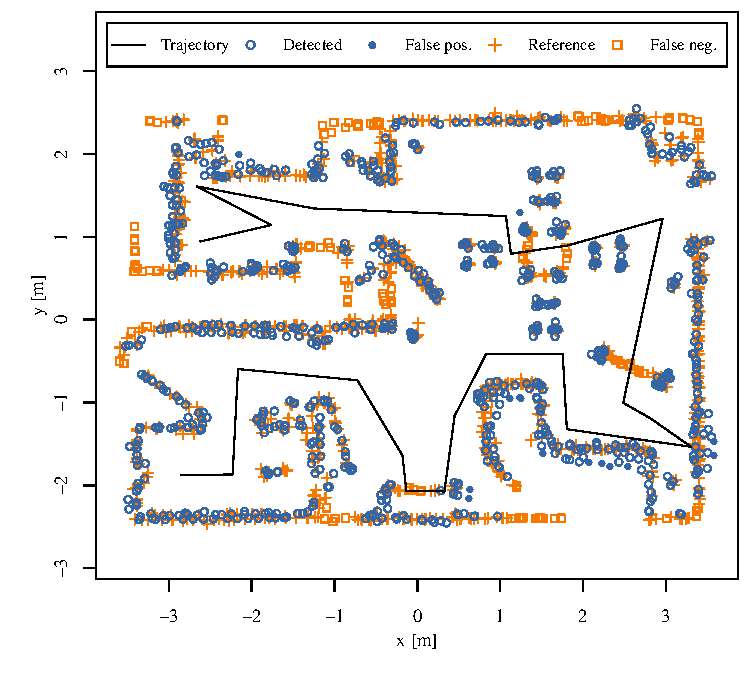
\includegraphics[width=0.975\textwidth]{results/simulation/apartment_overview.pdf}
  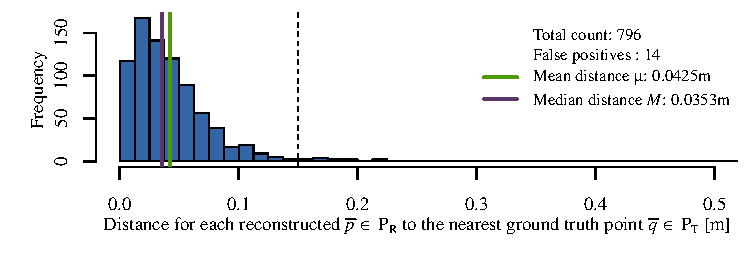
\includegraphics[width=0.975\textwidth]{results/simulation/apartment_histogram.pdf}
  \renewcommand{\arraystretch}{1.25}
  \begin{tabular}{l  l | l  l}
   Reconstructed count: & $796$ & Ground truth count: & $1150$ \\
   \hline
   False positives: & $14$ & True positive: & $782$ \\
   \hline
   $\nu_F$: & $1.76\%$ & $\nu_T$: & $68\%$ \\
   \hline
   $\mu$: & $0.0425 \,\mathrm{m}$ & $M$: & $0.0353 \,\mathrm{m}$ \\
   \hline
   $\mu_D$: & $0.594 \,\mathrm{m}$ & $M_D$: & $0.218 \,\mathrm{m}$ \\
   \hline
   Average time: & $24.28 \, \mathrm{ms}$ & Max. time:& $35.40 \, \mathrm{ms}$
  \end{tabular}
  \renewcommand{\arraystretch}{1}
 \end{center}
 \caption{Overall results for a simulated run in the apartment scene using the default parameters described above. See figure \ref{fig:floorplan} for the room layout.}
 \label{fig:simulation_result_apartment}
 \end{leftfullpage}
\end{figure}

\begin{figure}[p]
 \begin{fullpage}
 \begin{center}
  \textbf{Laboratory scene}\\
  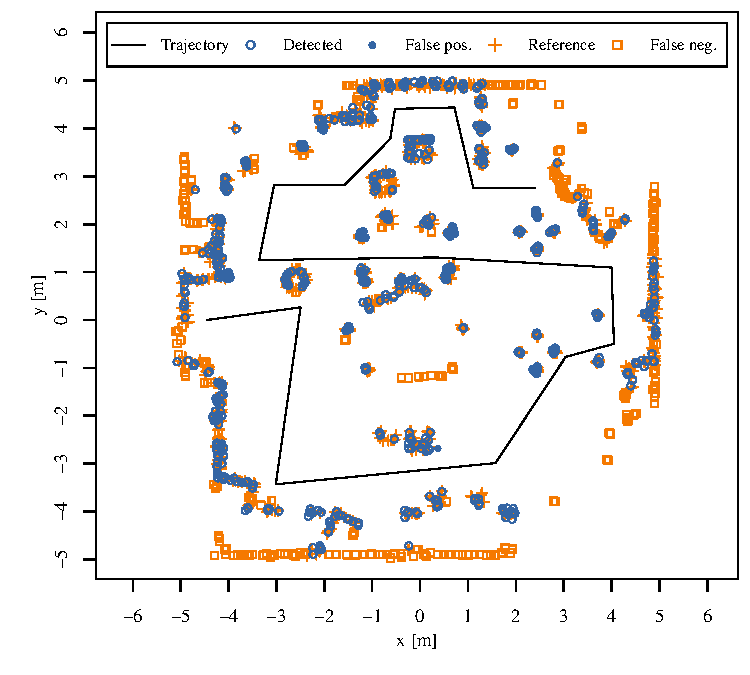
\includegraphics[width=0.975\textwidth]{results/simulation/laboratory_overview.pdf}
  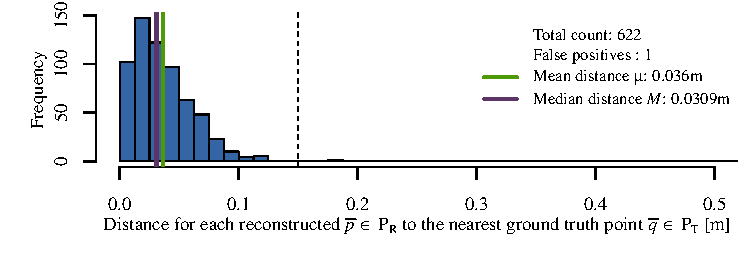
\includegraphics[width=0.975\textwidth]{results/simulation/laboratory_histogram.pdf}
  \renewcommand{\arraystretch}{1.25}
  \begin{tabular}{l  l | l  l}
   Reconstructed count: & $622$ & Ground truth count: & $1225$ \\
   \hline
   False positives: & $1$ & True positive: & $621$ \\
   \hline
   $\nu_F$: & $0.16\%$ & $\nu_T$: & $51\%$ \\
   \hline
   $\mu$: & $0.036 \,\mathrm{m}$ & $M$: & $0.0309 \,\mathrm{m}$ \\
   \hline
   $\mu_D$: & $0.769 \,\mathrm{m}$ & $M_D$: & $0.307 \,\mathrm{m}$ \\
   \hline
   Average time: & $16.39 \, \mathrm{ms}$ & Max. time:& $27.2 \, \mathrm{ms}$
  \end{tabular}
  \renewcommand{\arraystretch}{1}
 \end{center}
 \caption{Overall results for a simulated run in the laboratory scene using the default parameters described above. See figure \ref{fig:floorplan} for the room layout.}
 \label{fig:simulation_result_laboratory}
 \end{fullpage}
\end{figure}

%%%%%%%%%%% END DOUBLE PAGE %%%%%%%%%%%%%%%%

This section features a set of experiments in the environments described above and the corresponding results. First the overall results for both simulation and real-world tests are presented. Subsequent experiments seek to explore the impact of the error stack bias parameter $\tau$, the effects of coarse-to-fine refinement and the robustness against noise.

\subsection{Default parameters}

Unless noted differently, the following default parameters are used for both simulation and real-world tests:
\begin{description}
 \item[Input image:] $720 \times 96$ pixels, depression angle $\check \gamma = 0^\circ$, elevation angle $\hat \gamma = 30^\circ$, reduced elevation angle (region in which the depth is reconstructed) $\hat \gamma' = 10^\circ$.
 \item[Error stack calculation:] $32$ error stack layers (at $d = 0.04 \, \mathrm{m}$ $r_i$ ranges from $r_0 = \infty$ to $r_{31} \approx 0.15 \mathrm{m}$), error stack bias $\tau = 1$.
 \item[Coarse-to-fine refinement:] Search range $K = 2 \kappa + 1 = 8$; $3$ coarse-to-fine refinement steps.
 \item[Minimum error search:] $W_\vec{p}$ is a $3 \times 3$ binomial filter kernel, $\lambda = 1$, one refinement iteration.
 \item[Local environment map:] The standard deviation in depth direction is chosen as $\sigma_r = 0.01 \cdot (r^2 + 1 \, \mathrm{m}^2)$, the environment map density value threshold as $\eta = 40$.
\end{description}

\subsection{Simulated test run}

\paragraph{Experiment description:} In this experiment a test run with the default parameters (as given above) is conducted for each simulated environment. Runtime measurements are performed on an Intel\textregistered\ Atom\texttrademark\ N2600 dual core CPU running at $1{.}60 \, \mathrm{GHz}$ (the same model controlling the target robot) and covers both the depth reconstruction and the obstacle detection stage.

\paragraph{Results:} The results of this test run can be seen in figure \ref{fig:simulation_result_apartment} (apartment scene) and \ref{fig:simulation_result_laboratory} (laboratory scene), where \textit{false negative} obstacle points are defined as reference points $\vec q \in P_T$ with $\mathcal{D}(\vec q; P_R) > \chi$.


In the apartment scene, the algorithm creates multiple false positive obstacle points in the couch region and a single false positive point in the table region. On the other hand, all major obstacles are detected, including the table and chair legs. Most walls are detected. Relatively few obstacle points are detected for the brushed stainless steel refrigerator and the glass front of the stove (bottom right and top middle of the kitchen).

In the laboratory scene a single false positive obstacle point is found. Generally fewer obstacle points are detected (likely due to the size and higher sparsity of the room), yet all obstacles surrounding the trajectory in a distance of up to $1$ to $1.5 \,\mathrm{m}$ are detected. A notable exception is the checkerboard in the middle of the room.

During the simulation run it can be observed that the detection range is smaller for obstacles which lie in the direction of the focus of expansion or the focus of contraction, unless the corresponding objects have a prominent texture. For example at the end of the trajectory in the laboratory scene one can see that the (untextured) cylinders lying directly in front of the robot are not detected. With an average execution time of $24.28 \; \mathrm{ms}$ and $16.39 \; \mathrm{ms}$, respectively, real-time execution is possible on the target processor.

\subsection{Real-world test run}

\begin{figure}[t]
 \begin{center}
  \subbottom[Reconstructed obstacle points\label{fig:results_real1:a}]{
  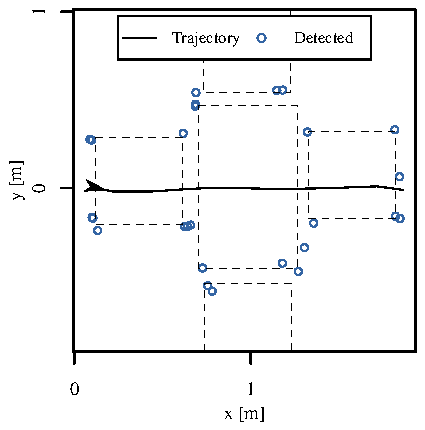
\includegraphics[width=0.475\textwidth]{results/real/obst5_furniture.pdf}
  }
  \subbottom[Local environment map\label{fig:results_real1:b}]{
  \raisebox{1.125cm}{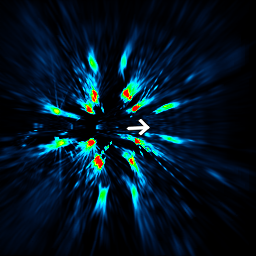
\includegraphics[width=0.385\textwidth]{results/real/obst5_map_ss.png}}
  }
  \subbottom[Depth reconstruction\label{fig:results_real1:c}]{
  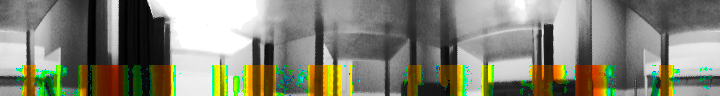
\includegraphics[width=0.85\textwidth]{results/real/obst5_depth_ss.png}
  }
  \subbottom[Artifacts introduced by tilting\label{fig:results_real1:d}]{
  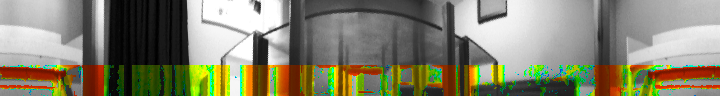
\includegraphics[width=0.85\textwidth]{results/real/obst5_depth2_ss.png}
  }
 \end{center}
 \caption{Test room dinner table results. (a) Obstacle points emitted during the test run and the corresponding trajectory (odometry data integration). The dashed lines depict the approximate position of the table and the four chairs (only shown for visualization and orientation purposes). (b) Local environment map. The arrow depicts the current robot position and orientation. (c) A snapshot of the depth reconstruction at the arrow position. Notice how the table legs are colored in yellow, orange and red depending on their distance. See figure \ref{fig:bias_depth_reconstruction} for details on the used color coding. (d) Artifacts in the depth reconstruction (note the red/near regions at the side and in the middle of the image) introduced by tilting the robot.}
 \label{fig:results_real1}
\end{figure}

\begin{figure}[t]
  \begin{center}
   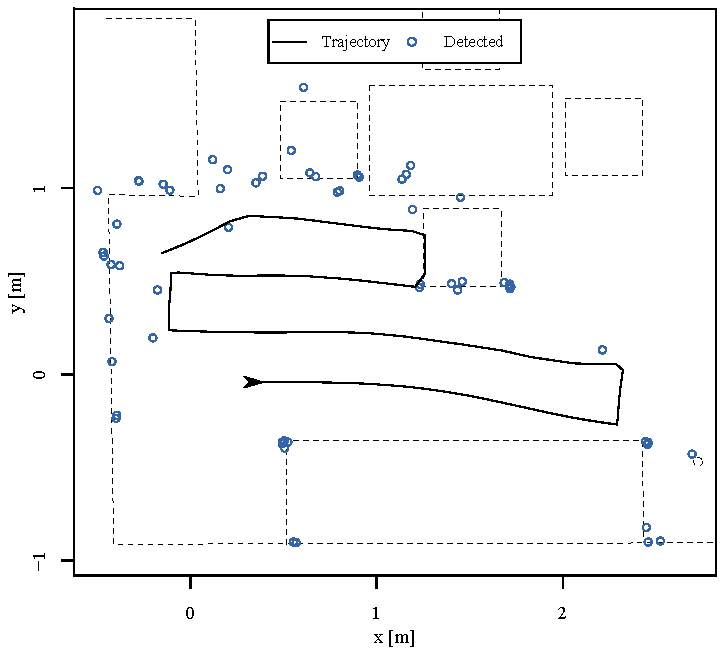
\includegraphics[width=0.975\textwidth]{results/real/obst6_furniture.pdf}
  \end{center}
  \caption{Test room results. Blue circles show obstacle points which were emitted during the test run, the straight line depicts the corresponding robot trajectory (odometry data integration). The dashed lines depict the approximate position of the furniture (table, four chairs, couch, sideboard) and the walls (only shown for visualization and orientation purposes). Note that the left wall is partially covered by a curtain.}
 \label{fig:results_real2}
\end{figure}

The results of two test runs in the test room environment described above can be seen in the figures \ref{fig:results_real1} and \ref{fig:results_real2}. Note that the environment map threshold $\eta$ (see section \ref{sec:obstacle_detection}) is doubled from $\eta = 40$ to $\eta = 80$ in order to increase the robustness against noise in exchange for a reduced detection range.

In the first test run, the robot drives a straight trajectory between the legs of the living room suite (see figure \ref{fig:results_real1:a}). The legs of chairs and tables are detected, although superimposed by relatively severe noise. In the depth reconstruction, the legs are correctly classified (figure \ref{fig:results_real1:c}), yet the depth of each leg spills onto background pixels. Correspondingly the probability distributions belonging to the table legs occupy relatively large regions in the local environment map (figure \ref{fig:results_real1:b}).

A false obstacle point is emitted at the end of the trajectory. At this position, the robot tilts/changes its elevation while driving over the edge of a carpet. Figure \ref{fig:results_real1:d} shows the corresponding artifacts in the depth map, which are responsible for the false positive obstacle point.

In the second test run, the legs of the couch (bottom region in figure \ref{fig:results_real2}) as well as the floor lamp to it's right are correctly detected. Correct obstacle points are also detected for the left wall which is partially covered by a curtain and two legs of the bottom chair. However, a large amount of false positive obstacle points is emitted in the top-left region of the trajectory.

\subsection{Error stack bias}

\begin{figure}[p]
 \begin{center}
  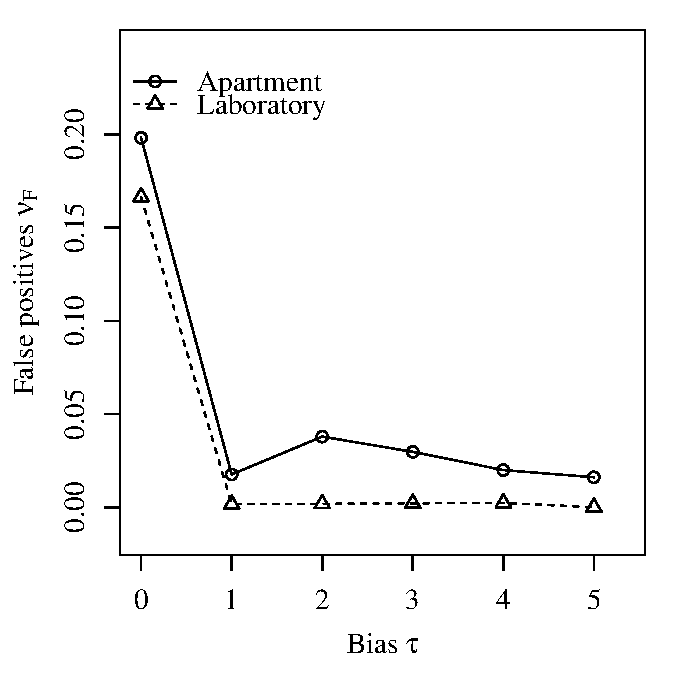
\includegraphics[width=0.44\textwidth]{results/bias/bias_mF.pdf}
  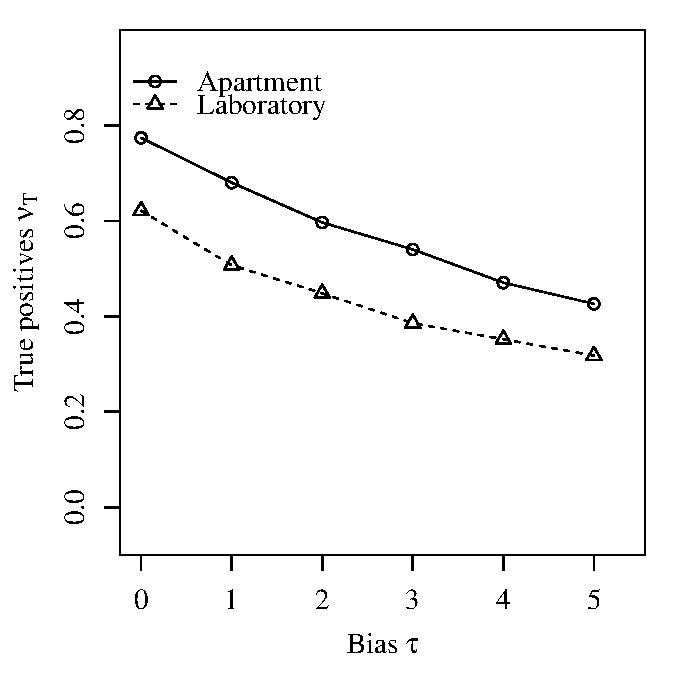
\includegraphics[width=0.44\textwidth]{results/bias/bias_mT.pdf}
  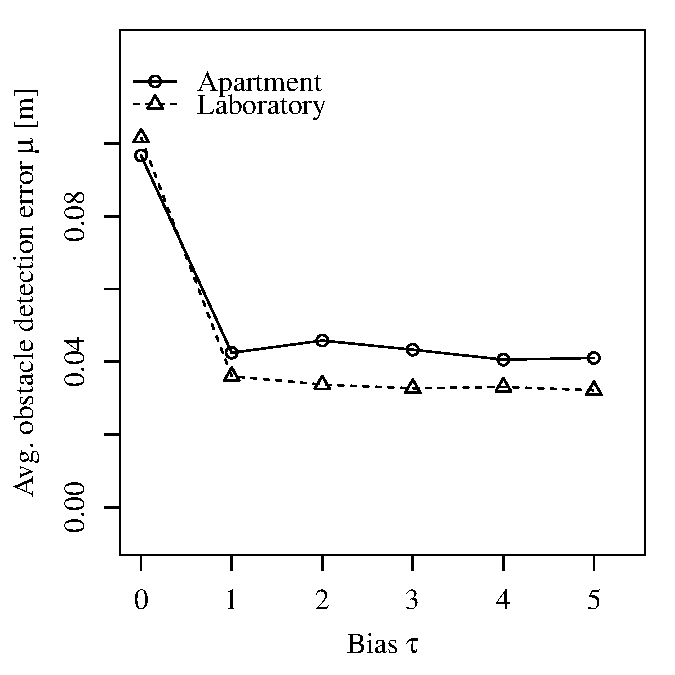
\includegraphics[width=0.44\textwidth]{results/bias/bias_meanDist.pdf}
  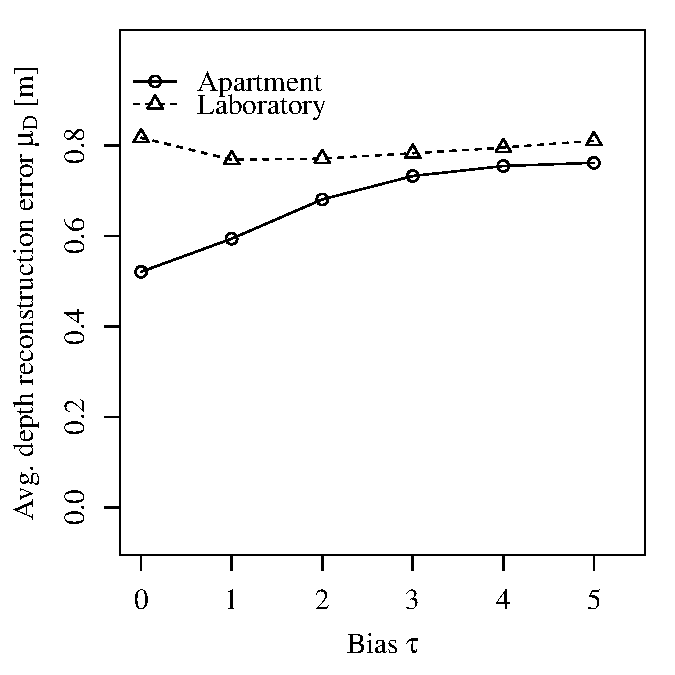
\includegraphics[width=0.44\textwidth]{results/bias/bias_avgNettoMean.pdf}
 \end{center}
 \caption{Results for varying the error stack bias $\tau$ for both the laboratory and the apartment scene.}
 \label{fig:results_bias}
\end{figure}

\begin{figure}[p]
\begin{center}
  \begin{tabular}{p{0.76\textwidth} p{0.085\textwidth}}
  \subbottom[$\tau = 0$]{
    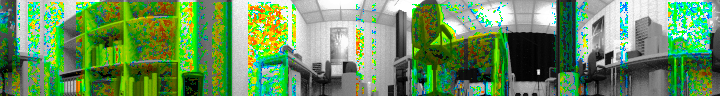
\includegraphics[width=0.75\textwidth]{results/bias/bias_off.png}
  }
  \subbottom[$\tau = 1$]{
    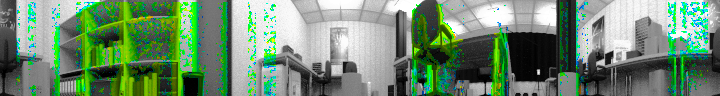
\includegraphics[width=0.75\textwidth]{results/bias/bias_on.png}
  }
  &
  \subbottom{
    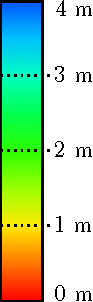
\includegraphics[width=0.084\textwidth]{media/depth_scale_vert.pdf}
  }
  \end{tabular}
\end{center}
\caption{Two depth reconstruction results for the laboratory scene for $\tau = 0$ and $\tau = 1$. For these particular images, the reduced elevation angle $\hat \gamma'$ was set to $\hat \gamma = 30^\circ$. Uncolored image regions either have a reconstructed distance larger than $4\,\mathrm{m}$ or were pruned in the coarse-to-fine refinement.}
\label{fig:bias_depth_reconstruction}
\end{figure}

\paragraph{Experiment description:} This test run measures the effect of the error stack bias parameter $\tau$ in the simulated environments (introduced in section \ref{sec:minimum_error_search}). The parameter $\tau$ is varied between $0$ and $5$. Due to restrictions in the optimized implementation only integral values are tested.

\paragraph{Results:} As shown in figure \ref{fig:results_bias}, nearly $\nicefrac{1}5$ of the reconstructed points are false positive for $\tau = 0$, in both laboratory scene and apartment scene. This number rapidly decreases as soon as $\tau \geq 1$. Yet a further increase in $\tau$ continuously decreases the count of reconstructed obstacle points as well as (at least in the apartment scene) the depth reconstruction error. Note how in the large laboratory room the depth reconstruction error decreases in the step from $\tau = 0$ to $\tau = 1$. The depth reconstruction result shown in figure \ref{fig:bias_depth_reconstruction} shows false classifications in unstructured areas of the input image for $\tau = 0$, which are eliminated for $\tau = 1$.

\subsection{Coarse-to-fine search}

\begin{figure}[t]
\begin{center}
 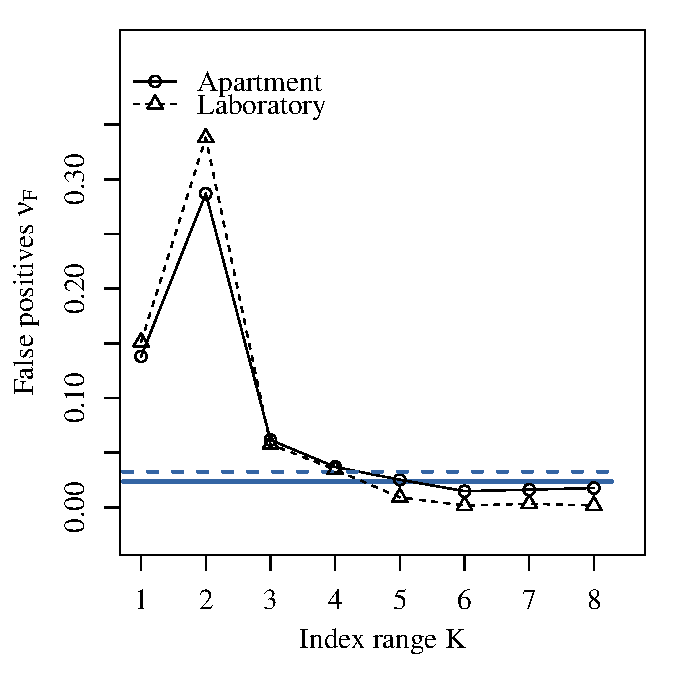
\includegraphics[width=0.475\textwidth]{results/index_range/idx_mF.pdf}
 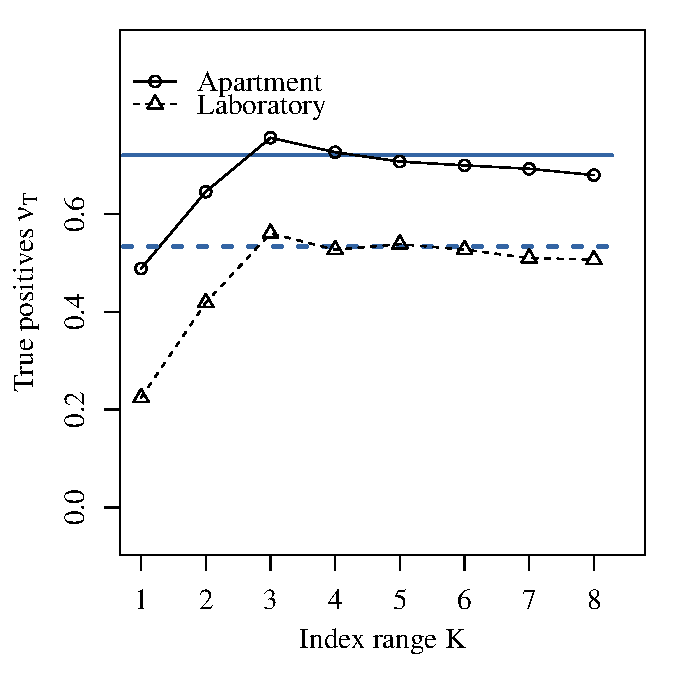
\includegraphics[width=0.475\textwidth]{results/index_range/idx_mT.pdf}
 %\includegraphics[width=0.475\textwidth]{results/index_range/idx_meanDist.pdf}
 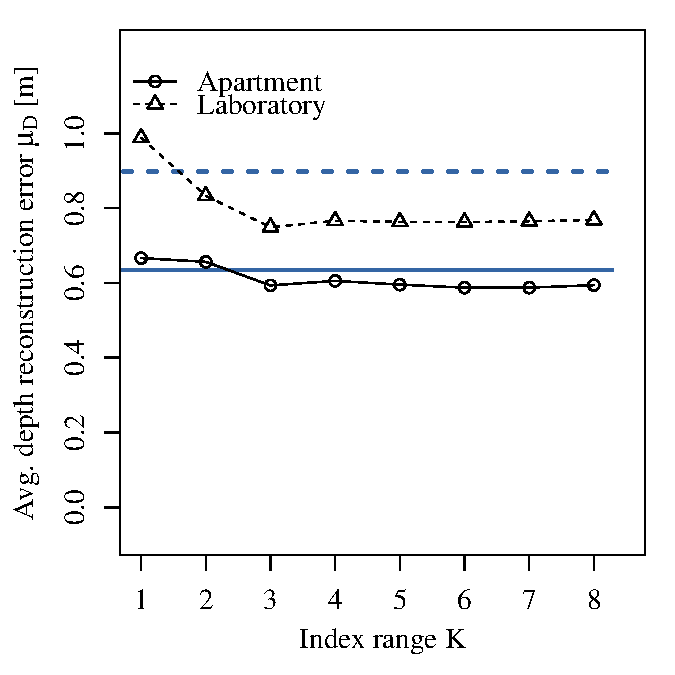
\includegraphics[width=0.475\textwidth]{results/index_range/idx_avgNettoMean.pdf}
 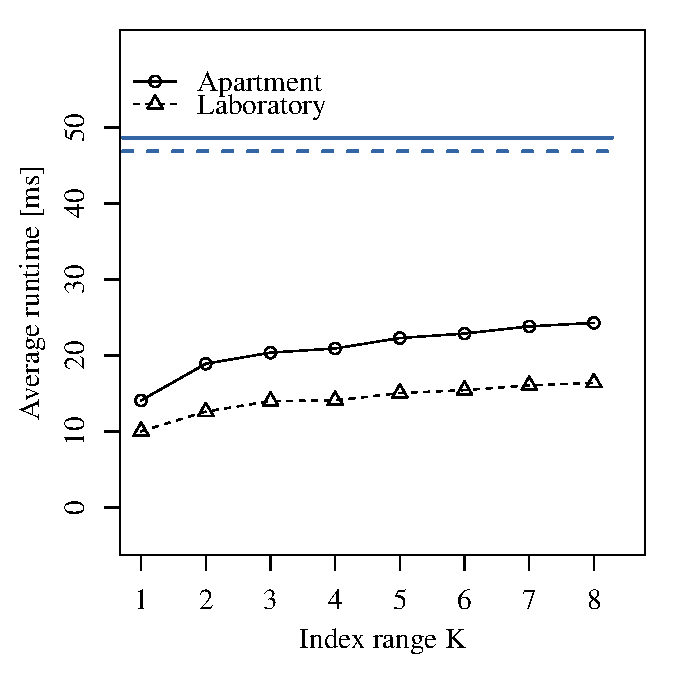
\includegraphics[width=0.475\textwidth]{results/index_range/idx_avgTime.pdf}
\end{center}
\caption{Results for varying index search range $K$ in both the apartment and the laboratory environment. The horizontal lines (blue) correspond to the result without coarse-to-fine refinement.}
\label{fig:results_index_range}
\end{figure}

\begin{figure}[t]
  \begin{center}
%  \subbottom[Reference run, no coarse-to-fine refinement]{
   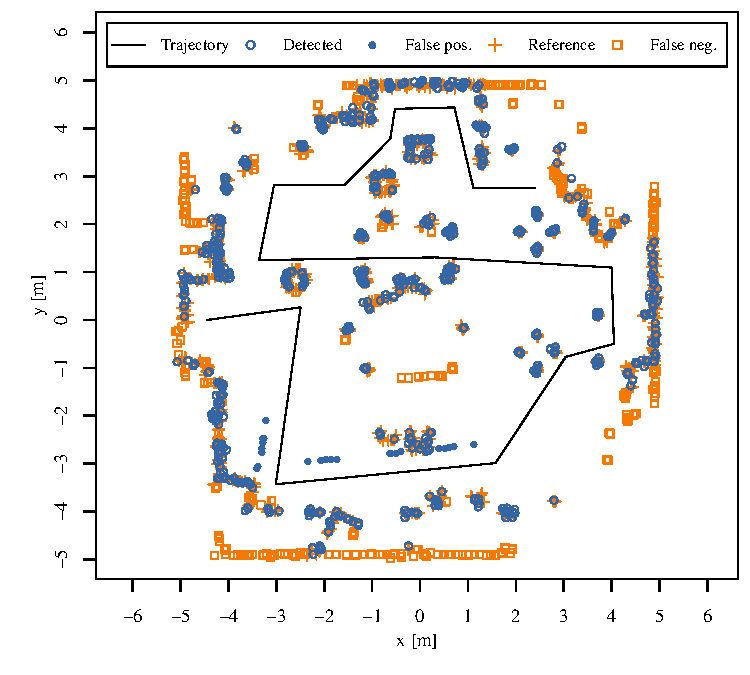
\includegraphics[width=0.975\textwidth]{results/index_range/overview_no_coarse_to_fine.pdf}
   %}
   %\subbottom[With coarse-to-fine refinement and $K = 8$]{
  % \includegraphics[width=0.75\textwidth]{results/index_range/overview_coarse_to_fine_8.pdf}
   %}
  \end{center}
  \caption{Obstacle detection performance in the simulated laboratory environment without coarse-to-fine refinement. Note the false positive points. See figure \ref{fig:floorplan} for a room plan and see figure \ref{fig:simulation_result_laboratory} for the run with coarse-to-fine refinement.}
  \label{fig:results_temporal_aliasing}
\end{figure}

\begin{figure}[t]
\begin{center}
  \subbottom[Without coarse-to-fine refinement]{
    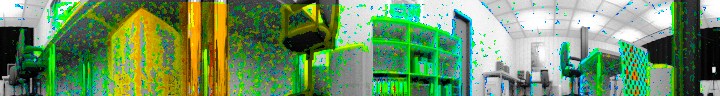
\includegraphics[width=0.75\textwidth]{results/index_range/index_range_off.png}
    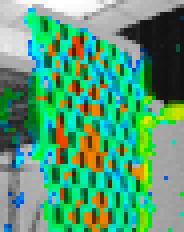
\includegraphics[width=0.08\textwidth]{results/index_range/small_no_coarse_to_fine.png}
  }
  \subbottom[Coarse-to-fine search, $K = 8$]{
    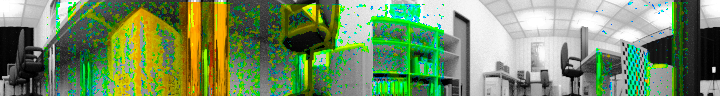
\includegraphics[width=0.75\textwidth]{results/index_range/index_range_on.png}
    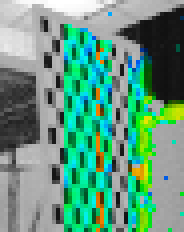
\includegraphics[width=0.08\textwidth]{results/index_range/small_coarse_to_fine.png}
  }
\end{center}
\caption{Two depth reconstruction results for the laboratory scene for the reference run (without coarse-to-fine refinement) (a) and with coarse-to-fine-search, $K = 8$ (b). The right images show the enlarged chess-board area. See figure \ref{fig:bias_depth_reconstruction} for details on the used color coding.}
\label{fig:coarse_to_fine_depth_reconstruction}
\end{figure}

\paragraph{Experiment description:} In this simulated test run the effects of the coarse-to-fine refinement on runtime and quality are to be measured.

The algorithm is executed in the apartment and laboratory test environments under different search range breadths $K \in \{1, \ldots, 8\}$. A reference run is performed in which coarse-to-fine refinement is disabled.

\paragraph{Results:} The result of the test runs is shown in figure \ref{fig:results_index_range}: One can see, that in comparison to the reference run, the depth reconstruction error $\mu_D$ is reduced for $K \geq 3$. The same is true for the false positive count $\nu_F$, yet a search range of $K = 6$ is required in order to perform considerably better in the apartment scene. For large search ranges the true positive count $\nu_T$ is slightly reduced compared to the reference value.

The runtime rises with increasing search range, yet even for $K = 8$ the total runtime is reduced by nearly $50\%$ compared to the reference run.

Figure \ref{fig:results_temporal_aliasing} shows detected and reference obstacle points as a global top-down map in the laboratory environment without coarse-to-fine refinement. In contrast to the result shown in figure \ref{fig:simulation_result_laboratory} (which had coarse-to-fine refinement enabled), false positive obstacle points are detected in the lower left region. This region features repeating patterns including a bookshelf and a chess board, see second laboratory snapshot example image in figure \ref{fig:sample_snapshots}. Figure \ref{fig:coarse_to_fine_depth_reconstruction} shows a snapshot of the depth reconstruction for that region, with both enabled and disabled coarse-to-fine refinement. One can see, that the coarse-to-fine refinement eliminates the artifacts in the depth map, which are suspected to cause the false positive obstacle points.

\subsection{Noise robustness}

\label{sec:noise}

\begin{figure}[p]
 \begin{center}
  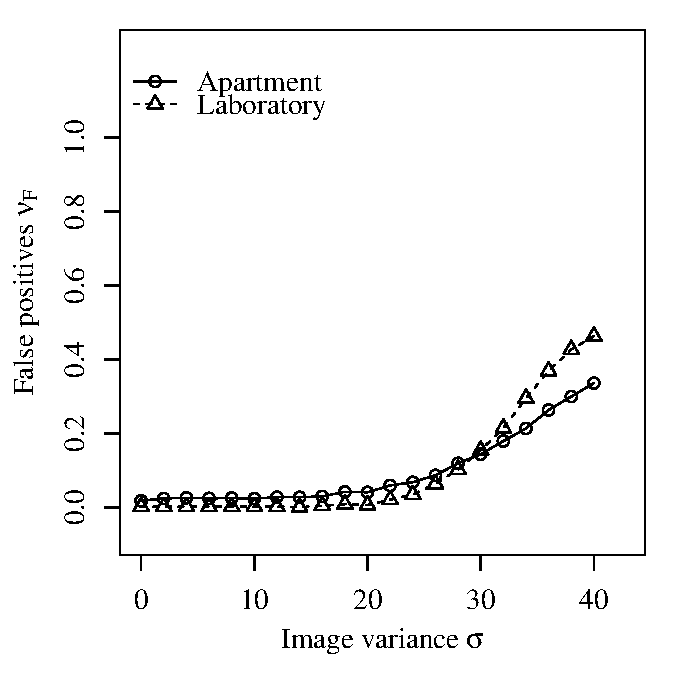
\includegraphics[width=0.475\textwidth]{results/noise/noise_image_mF.pdf}
  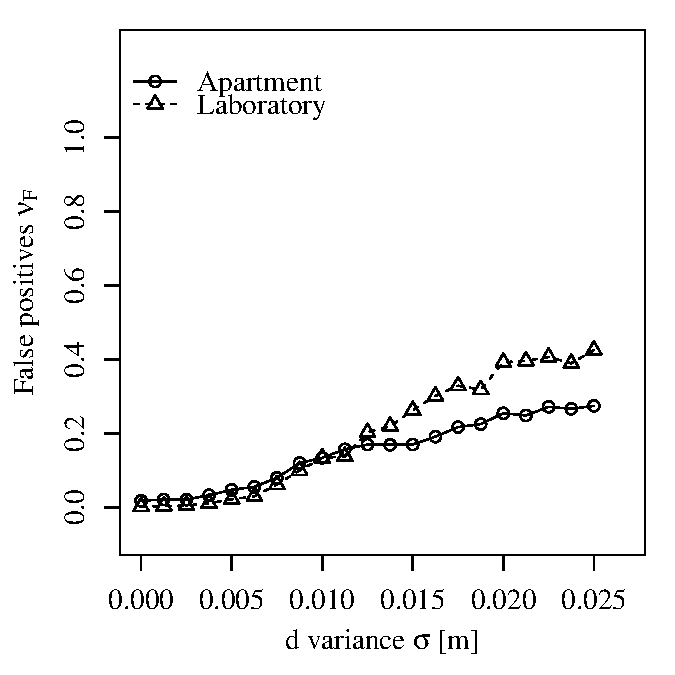
\includegraphics[width=0.475\textwidth]{results/noise/noise_d_mF.pdf}
  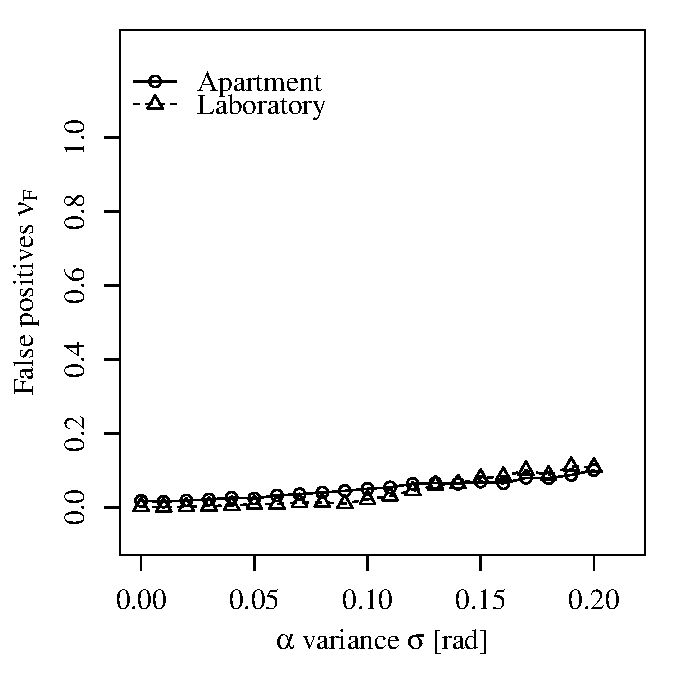
\includegraphics[width=0.475\textwidth]{results/noise/noise_alpha_mF.pdf}
  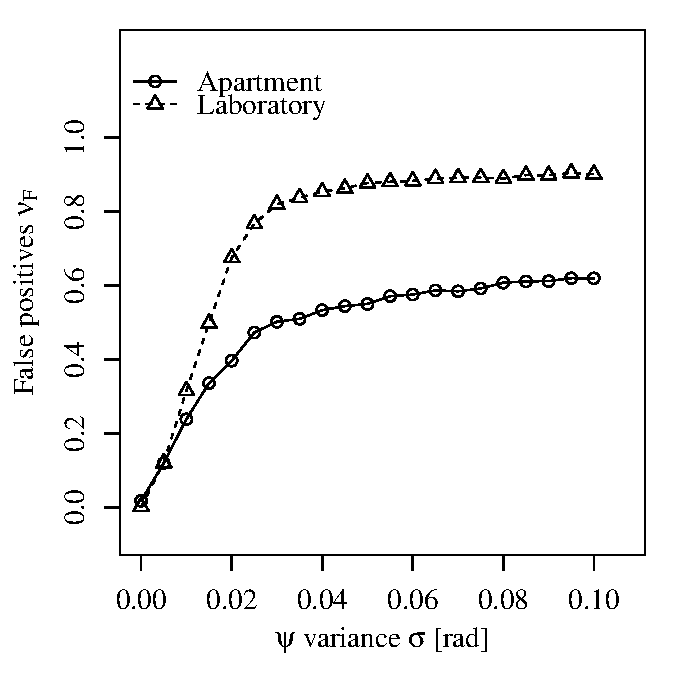
\includegraphics[width=0.475\textwidth]{results/noise/noise_psi_mF.pdf}
 \end{center}
 \caption{Impact of noise superimposed on the input images and the motion parameters on the relative false positive count $\nu_F$ for both the laboratory and the apartment scene.}
 \label{fig:results_noise}
\end{figure}

\begin{figure}[p]
 \begin{center}
  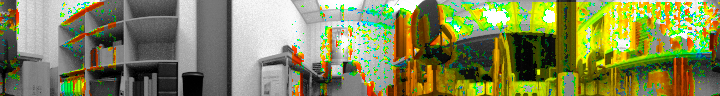
\includegraphics[width=0.85\textwidth]{results/noise/noise_depth_psi.png}
 \end{center}
 \caption{Depth reconstruction result for the laboratory scene showing artifacts introduced by a $0.0287$ radians ($1.64^\circ$) deviation of $\psi$. See figure \ref{fig:bias_depth_reconstruction} for details on the used color coding and the reference result.}
 \label{fig:noise_depth_reconstruction}
\end{figure}

\paragraph{Experiment description:} In this test, the impact of noisy input data is measured. The noise leads to violations of the assumptions made in section \ref{sec:assumptions}. The input data (motion parameters $d, \alpha$ and $\psi$, as well as the input image $\img{I}$) are superimposed by an additive Gaussian noise term with standard deviation $\sigma$. The noise is sampled independently at each data point/pixel.

The following (arbitrarily chosen) standard deviations are used: For $d$ (traveled distance) $\sigma$ is varied from $\sigma = 0 \, \mathrm{m}$ to $\sigma = 0.025 \, \mathrm{m}$ (the relative error at $d = 0.04$ ranges from $0\%$ to $62.5\%$). For $\alpha$ (motion direction) $\sigma$ is varied from $\sigma = 0 $ to $\sigma = 0.2$ radians (in degrees: $0^\circ$ to $11.46^\circ$). For $\psi$ (change in orientation) $\sigma$ is varied from $\sigma = 0 $ to $\sigma = 0.1$ (in degrees: $0^\circ$ to $5.73^\circ$). For the image $\img{I}$ the standard deviation is varied from $\sigma = 0$ to $\sigma = 40$ (relative deviation ranges from $0\%$ to $16\%$ for 8-bit intensity values). In all experiments $\sigma$ is varied in 20 steps.

\paragraph{Results:} The results presented in figure \ref{fig:results_noise} show that independent noise superimposed on the input image and the motion parameters $\alpha$ and $d$ only has a very subtle impact on the count of false positive obstacles until certain thresholds are reached: Image noise starts to effect the output noticeably at $\sigma \approx 20$ ($8\%$), noise in $d$ is is tolerable up to $\sigma \approx 0.005 \, \mathrm{m}$ ($12.5\%$) and noise in $\alpha$ has only little effect on the false positive count for deviations up to $\sigma \approx 0.1$ radians ($5.73^\circ$). However, even small deviations in the orientation change $\psi$ result in a high false positive count: Even a deviation of $0.02$ radians ($\approx 1^\circ$) causes almost every second reconstructed obstacle point to be false positive. See figure \ref{fig:noise_depth_reconstruction} for the impact of noisy $\psi$ on the depth reconstruction.
